\documentclass[a4paper]{article}
\usepackage{amsmath}
\usepackage{amsfonts}
\usepackage{amssymb}
\usepackage{graphicx}
\usepackage{float}

\begin{document}

\noindent \large Auteur: Siebe Haché \\
\noindent \large Studierichting: Informatica \\
\noindent \large Oefeningenreeks 5D nr. 14 \\

\medskip
\normalsize

Bereken de oppervlakte ingesloten door de lus van de kromme $y^2 = x^4 + x^5$. \\

De nulpunten zijn $x = 0$ en $x = -1$. De lus bevindt zich op het interval $[-1, 0]$ \\

$S = 2 \displaystyle\int_{-1}^{0} \sqrt{x^4 + x^5} dx$ \\

$= 2 \displaystyle\int_{-1}^{0} \sqrt{x^4(1 + x)} dx$ \\

$= 2 \displaystyle\int_{-1}^{0} x^2 \sqrt{1 + x} dx$ \\

Stel $u = 1+x$:\\

$S = 2 \displaystyle\int_{0}^{1} (u-1)^2 \sqrt{u} du$ \\

$= 2 \displaystyle\int_{0}^{1} (u^2 - 2u + 1) u^{1/2} du$ \\

$= 2 \displaystyle\int_{0}^{1} (u^{5/2} - 2u^{3/2} + u^{1/2}) du$ \\

$= 2 \left[\dfrac{2}{7}u^{7/2} - 2 \cdot\dfrac{2}{5}u^{5/2} + \dfrac{2}{3}u^{3/2} \right]_{0}^{1}$ \\

$= 2 \left(\dfrac{2}{7} -\dfrac{4}{5}+ \dfrac{2}{3} \right)$ \\

$= 2 \left( \dfrac{30 - 84 + 70}{105} \right)$ \\

$= 2 \left( \dfrac{16}{105} \right) = \dfrac{32}{105}$ \\

\begin{figure}[H]
    \centering
    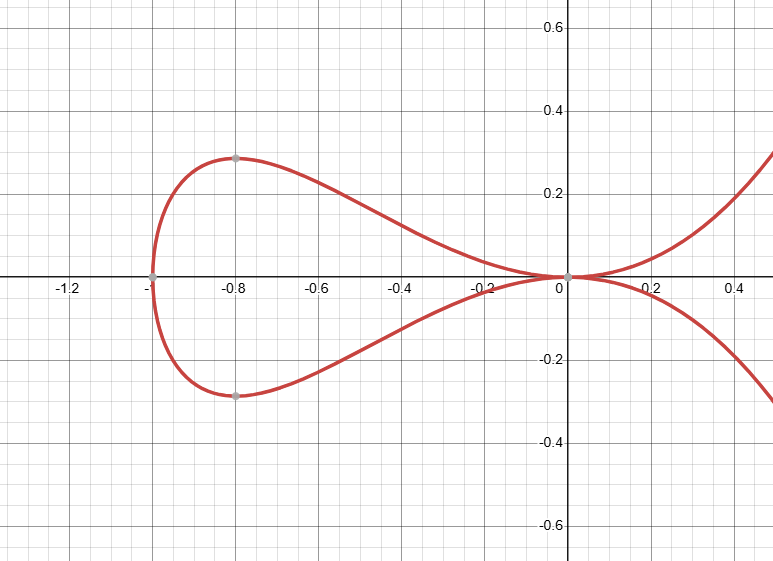
\includegraphics[width=0.6\textwidth]{5D-14-siebe.hache.INF.png}
\end{figure}

\begin{thebibliography}{999}
\bibitem{a} Grafiek gemaakt met Desmos.com
\end{thebibliography}
\end{document}